%%This is a very basic article template.
%%There is just one section and two subsections.
\documentclass[fleqn]{article}
\usepackage{amsmath}					%Math formats
\usepackage{amssymb}					%More math formats
\usepackage{lastpage}					%Page number computation
\usepackage{fancyhdr}					%For headers
\usepackage[margin=0.75in]{geometry}	%better margins
\usepackage{pdfpages}					%include pdfs
\usepackage{graphicx}

\newcommand{\mm}[1]{\begin{pmatrix}#1\end{pmatrix}}
\newcommand{\nn}[1]{ \begin{align*}#1\end{align*}}
\newcommand{\cc}[1]{}

\pagestyle{fancy}
\fancyhf{} 
\fancyhead[LE,RO]{Homework 3 - Greg Timmons}
\fancyhead[RE,LO]{CSC 579 - Perf Modeling}
\fancypagestyle{plain}{\fancyfoot[LE,RO]{\thepage\backslash\pageref{LastPage}}} 
\fancyfoot[LE,RO]{\thepage\backslash\pageref{LastPage}}  

\begin{document}

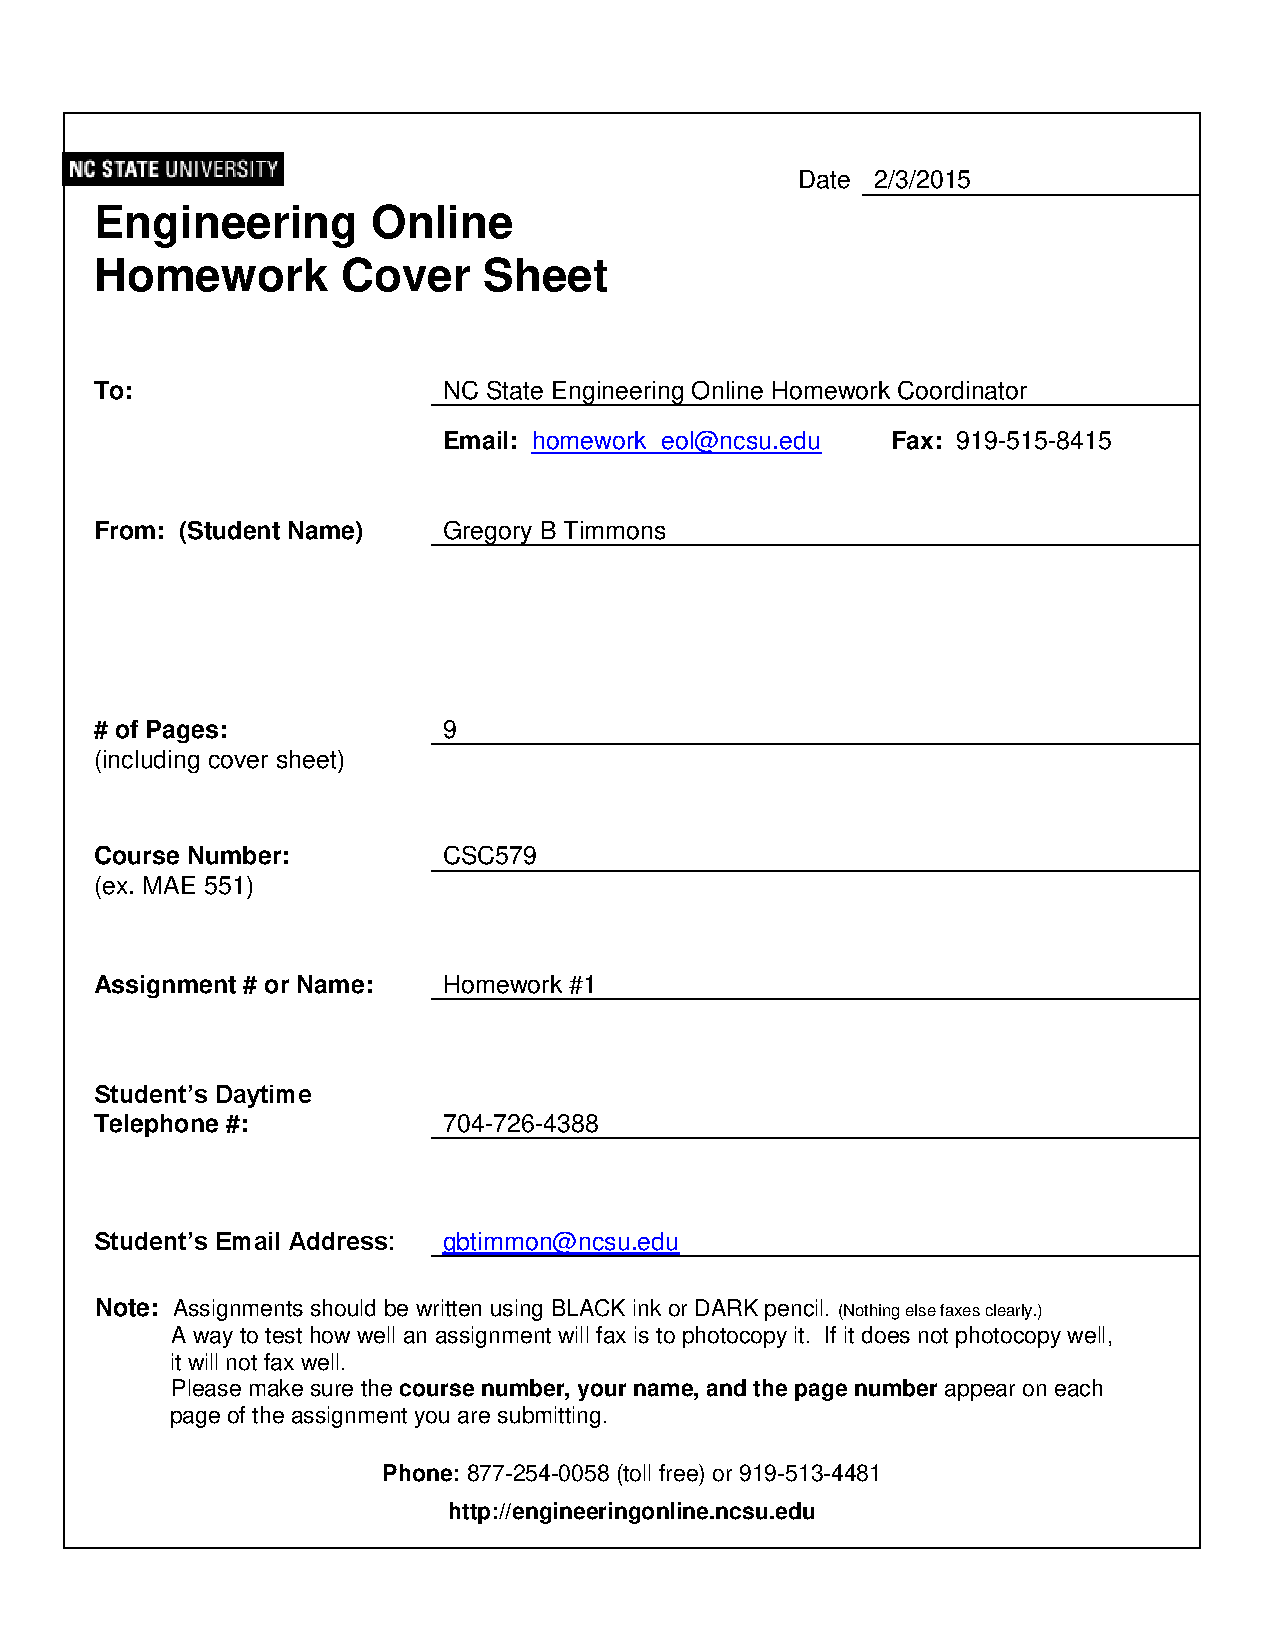
\includepdf[pages={1}]{cover.pdf}
\title{Homework 3}
\date{April 16, 2015}
\author{Gregory B Timmons, gbtimmon}
\maketitle

\section*{Question 1}	
\nn{ 
	\lambda 	&= 1,\\
	\alpha_1 	&= 0.5,\ \alpha_2 = 0.3,\ \alpha_3 = 0.2,\\
	\mu_1 		&= 4,\ \mu_2 = 2,\ \mu_3 = 1 
}

\begin{figure}[ht!]
\includegraphics[width=90mm]{STD_Question1.jpg}
\end{figure}
We have a QBD process and will compute Nuets R Matrix. 
\nn{\mm{
  	B_{00} & B_{01} & 0 & 0 & \ldots\\
  	B_{10} & A_1 & A_2 & 0  & \ldots\\ 
  	0      & A_0 & A_1 & A_2 & \ldots\\ 
  	0      & 0   & A_0 & A_1 & \ldots\\
 	\vdots&\vdots&\vdots&\vdots&\ddots 
 }}
 
\nn{
	B_{00} 	&= \mm{-\lambda}\quad \\
  	B_{01} 	&= \mm{\alpha_1\lambda & \alpha_2\lambda &\alpha_3\lambda}\\
  	B_{10} 	&= \mm{\mu_1\\\mu_2\\\mu_3} \\
	A_{0} 	&= \mm{
		\alpha_1\mu_1&\alpha_2\mu_1&\alpha_3\mu_1\\
		\alpha_1\mu_2&\alpha_2\mu_2&\alpha_3\mu_2\\
		\alpha_1\mu_3&\alpha_2\mu_3&\alpha_3\mu_3\\
	} \\
	A_{1} 	&= \mm{
		-(\mu_1 + \lambda) \\
		&-(\mu_2+\lambda)\\
		&&-(\mu_3 +\lambda)} \\
	A_{2} 	&= \mm{
		\lambda\\
		&\lambda\\
		&&\lambda
	}
}
Values : 
\nn { 
	A_{0} &= \mm{2&1.2&.8\\1& .6&.4\\.5& .3&.2}\\ 
   	A_{1} &= \mm{-6\\&-4\\&&-3} \\
   	A_{2} &= \mm{2\\&2\\&&2}     
}
V and W :
\nn{
	V &= A_2A_1^{-1} =\mm{-2/6\\&-2/4\\&&-2/3} \\
	W &= A_0A_1^{-1} =\mm{-1/3&-3/10&-4/15\\-1/6&-3/20&-4/30\\-1/12&-3/40&-4/60}
}
Now we compute Nuets R Matrix ( first 2 iterations) :
\nn{
	R_{(k+1)} &= -V - R^2_{(k)}\\
	R_0 &=\mm{0&0&0\\0&0&0\\0&0&0}\\
	R_1 &= -V -R_{(0)}^{2}W =\boxed{\mm{1/6\\&1/4\\&&1/3}}\\
	R_2 &= -V -R^2_{(1)}W = \mm{2/6\\&2/4\\&&2/3} - \mm{1/6\\&1/4\\&&1/3}^2
    \mm{-1/3&-3/10&-4/15\\-1/6&-3/20&-4/30\\-1/12&-3/40&-4/60}
    =\boxed{\mm{
	    .370  &  .033 &   .029 \\
	    .041 &   .537 &   .033 \\
	    .037 &   .033 &   .696
	 }}}
  
 \section*{Question 2}
\nn{
	 \mm{ \pi_0 & \pi_1 & \pi_2 & \pi_3 & \ldots }
	 \mm{
	  	B_{00} & B_{01} & 0 & 0 & \ldots\\
	  	B_{10} & A_1 & A_2 & 0  & \ldots\\ 
	  	0      & A_0 & A_1 & A_2 & \ldots\\ 
	  	0      & 0   & A_0 & A_1 & \ldots\\
	 	\vdots&\vdots&\vdots&\vdots&\ddots  
	 } = (0) 
}
This give us the following system of equations
\nn{
	\mm{\pi_0&\pi_1}\ \mm{
		 B_{00} & B_{01} \\ 
		 B_{10} & A_{1} + R * A_{0}
	}=\mm{0&0}
}
Or Explicitly 
\nn{
	\mm{\pi_{0} & \pi_{1_0} & \pi_{1_1} & \pi_{1_2}} 
 	\mm{-2&1&0.6&0.4\\ 4&-5&.6&.4\\2&1&-3.4&.4\\1&1&.6&-2.6} = \mm{0&0&0&0}
}
In order to get an exact solution we make the following small adjustments : 
 \nn{
 	\mm{\pi_{0} & \pi_{1_0} & \pi_{1_1} & \pi_{1_2}} 
 	\mm{-2&1&0.6&1\\ 4&-5&.6&0\\2&1&-3.4&0\\1&1&.6&0} = \mm{0&0&0&1}
 }
 
Which gives us
\nn{
    \pi   &= \mm{ 1&1&0.6&0} \\
    \pi_0 &= \mm{1}, \\
    \pi_1 &= \mm{1&0.6&0}
}

Next solve for $\alpha$ 
\nn{
    \alpha &= \pi_0 e  + \pi_1( I - R )^{-1}e = 24.59\\
    \pi_0 &= \mm{0.04066}\\
    \pi_1 &= \mm{0.04065 & 0.0243 & 0 }\\
    \pi_{(k+1)} &= \pi_{1}R^{k-1} 
}
 
Now we have the values to compute the values we are
looking for $\alpha$
\nn{
     p_0           &= ||\pi_{0}||_1 = \boxed{ 0.04066 } \\
     p_3           &= ||\pi_1R^2||_1 = \boxed { 0.03798 } \\
     p\{n \geq 4\} &= ||\pi_1R^{3}(I-R)^{-1}||_1 = 0.8094 \ \mbox{or}\\
      &=1 - p_0 - p_1 - p_2 - p_3 = 1 - ||\pi_{0}||_1 -
    ||\pi_{1}||_1 - ||\pi_{1}R||_1 - ||\pi_{1}||_1 =\boxed{0.8094}
 }
\subsection*{Question 3}
Arrival Time 
\nn{
	E[X] 	&= 16 \\
	Var(X) 	&= 32 \\
	C^2_X 	&= Var(X)/E[X]^2 = 1/8 
}
Departure Time
\nn{
	E[Y] 	&= \mu^{-1} = 12/60 
}
We need to build a distribution to model this arrival pattern.
\nn{
	r 		&= \lceil \frac{1}{(1/8)} \rceil\\
			&= \boxed{8}\\
	\alpha 	&=\frac{r - 2C_X^2 + \sqrt{r^2 + 4 -4rC_X^2}}{2(C_X^2 + 1)(r-1)}\\
			&=\frac{8 - 2C_X^2 + \sqrt{68 -32C_X^2}}{14C_X^2 + 14)} \\
			&=\frac{8 - 2(1/8)^2 + \sqrt{68 -32(1/8)^2}}{14(1/8)^2 + 14)} \\
			&= \boxed{1}\\
	\mu 	&= \frac{1 + 1(8-1)}{16}\\
			&= \boxed{1/2}
}
This suggests we can simulate this with a Erlang-8 distribution, $mu = .5$.\\
Checking the work:
\nn{
	E[X]	&= (1-\alpha)\frac{1}{\mu} + \alpha\frac{r}{\mu}\\
			&= (0) + \frac{8}{.5}\\
			&= 16\\
	Var[X] 	&= \frac{2(1-\alpha)+\alpha r(r+1)-(1-\alpha+\alpha r)^2}{\mu^2}\\
			&= \frac{2(1-1)+ 8(8+1)-(1-1+8)^2}{(.5)^2} \\
			&= \frac{72 - 64}{.25}\\
			&= 32
	}
The question can be modeled as a $E_r/M/1$ with $\lambda = 1/2, r = 8,$ and $
\mu = 1/12$ 
\nn{
	B_{00} &= \mm{
		-.5 & .5& 0 &\ldots\\
		0 & -.5& .5 &\ldots\\
		0 & 0& -.5 &\ldots\\	
		\vdots&\vdots&\vdots&	
	}\\
	B_{01} &= \mm{
		\vdots&\vdots&\vdots&\\
		0&0&0&\ldots\\
		0&0&0&\ldots\\
		.5&0&0&\ldots\\
	}\\
	B_{10} &=\mm{
		1/12 & 0 & 0 &\ldots\\
		0 & 1/12 & 0 &\ldots\\
		0 & 0& 1/12 &\ldots\\	
		\vdots&\vdots&\vdots&	
	}\\
	A_0 &= B_{10}\\
	A_2 &= B_{01}\\
	A_1 &= \mm{
		-(1/2+1/12) & .5& 0 &\ldots\\
		0 & -(1/2+1/12)& .5 &\ldots\\
		0 & 0& -(1/2+1/12) &\ldots\\	
		\vdots&\vdots&\vdots&	
	}
}

Using matlab code we compute the following attributes of this Ph/Ph/1 Queue. 
\nn{
	R &= \mm{
	  0 &       0 &       0 &       0 &       0 &       0 &       0 &       0\\
      0 &       0 &       0 &       0 &       0 &       0 &       0 &       0\\
      0 &       0 &       0 &       0 &       0 &       0 &       0 &       0\\
      0 &       0 &       0 &       0 &       0 &       0 &       0 &       0\\
      0 &       0 &       0 &       0 &       0 &       0 &       0 &       0\\
      0 &       0 &       0 &       0 &       0 &       0 &       0 &       0\\
      0 &       0 &       0 &       0 &       0 &       0 &       0 &       0\\
 0.9357 &  0.8755 &  0.8191 &  0.7664 &  0.7171 &  0.6710 &  0.6278 & 0.5874
  }\\
  \pi_0 &=\mm{0.0080 &  0.0156&   0.0226 &  0.0292 &  0.0354& 0.0411& 0.0465& 0.0516}\\
  \pi_1 &=\mm{0.0483& 0.0452& 0.0422& 0.0395& 0.0370& 0.0346& 0.0324 &0.0303 }
}

Now to compute the desired metrics: \\
\nn{
	p\{N_q \geq 2\} &= p\{N \geq 3\} \\
					&= || \pi_1 R^{2}(I-R)^{-1}||_1\\
					&= \boxed{0.2588}\\
	E[N] 			&= ||\pi_1(I-R)^-2||_1\\
					&= \boxed{1.8178}\\
	E[N_q]			&= E[N] - \lambda/\mu\\
					&= 1.8178 - 0.75\\
					&= 1.0678\\
	E[R]			&= E[R] = E[N]/\lambda \\
					&= \boxed{29.0848}
}

\section*{Question 4}
a.)
\nn{
	P(z) 	&= \frac{1 + z^4}{10} + \frac{z + z^2 + z^3}{5}\\
			&= \frac{1}{10}+\frac{z}{5}+\frac{z^2}{5}+\frac{z^3}{5}+\frac{z^4}{10} \\
			&= .1 + .2z + .2z^2 + .2z^3 + .1z^4\\
	\Rightarrow p&=\{\frac{1}{10},\frac{1}{5},\frac{1}{5},\frac{1}{5},\frac{1}{10}\} 
} 
b.)
\nn{
	p_k		&= \frac{1}{k!}\frac{\partial^k}{\partial z^k}P(z)\vline_{z=0}
}\nn{
	p_0 	&= \frac{1}{0!}P(z)\vline_{z=0}\\
			&= \frac{1}{10}+\frac{0}{5}+\frac{0}{5}+\frac{0}{5}+\frac{0}{10}\\
			&= \boxed{\frac{1}{10}}
}\nn{
	p_1		&= \frac{1}{1!}\frac{\partial}{\partial z}P(z)\vline_{z=0}\\
			&= \frac{1}{5}(2z^3 + 3z^2 + 2z + 1)\vline_{z=0}\\
			&= \boxed{\frac{1}{5}}
}\nn{
	p_2 	&= \frac{1}{2!}\frac{\partial^2}{\partial z^2}P(z)\vline_{z=0}\\
			&= \frac{1}{2}*\frac{1}{5}(6z^2 + 6z + 2)\vline_{z=0}\\
			&= \boxed{\frac{1}{5}}
}\nn{
	p_3		&= \frac{1}{3!}\frac{\partial^3}{\partial z^3}P(z)\vline_{z=0}\\
			&= \frac{1}{6}*\frac{1}{5}(12z + 6)\vline_{z=0}\\
			&= \boxed{\frac{1}{5}}
}\nn{
	p_4		&= \frac{1}{4!}\frac{\partial^4}{\partial z^4}P(z)\vline_{z=0}\\
			&= \frac{1}{24}*\frac{12}{5}\vline_{z=0}\\
			&= \boxed{\frac{1}{10}}
}


\section*{Question 5}
a.)
\nn{
	g_i &\equiv \mbox{Prob}\{\mbox{Bulk size is i}\}\\
}
Balence Equation: 
\nn{
	(\lambda + \mu)p_k &= \mu p_{k+1} + \sum_{i=0}^{k-1}p_i\lambda g_{k-i}
}
\underline{Justification : }\\
Left Hand Side : \\
The rate of leaving a state by customer arrival is equal to lambda as shown
since the following equation holds $\lambda &= \lambda\sum_{i=0}^{\infty}g_i$. The rate of
leaving a state by customer departure is equal to a simple $\mu$.\\
\\
Right Hand Side : \\
The rate of entering a state by customer departure is the probability of being
in the state about that one by mu. The probability of entering a state by
costumer arrival is the probability of being a state $k - i$ by the probability
of a bulk of i members arriving ($g_i$).
\\\\
Forming the Z-Transforms : \\
\nn{
	(\lambda + \mu)\sum_{k=1}^{\infty}{p_k z^k} &=
	\mu z^{-1}\sum_{k=1}^{\infty}p_{k+1}z^{k+1} +
	\sum_{k=1}^{\infty}{\sum_{i=0}^{k-1}{p_i\lambda g_{k-i}z^k }}\\
	(\lambda + \mu)\sum_{k=1}^{\infty}{p_k z^k} &=
	\mu z^{-1}\sum_{k=1}^{\infty}p_{k+1}z^{k+1} + \lambda\sum_{i=0}^{\infty}{p_i
	z^i}\sum_{j=1}^{\infty}g_j z^j
}
Let $G(z)$ be the z-trasformation of the bulk arrival distributions :
\nn{
	G(z) &\equiv \sum_{k=1}^{\infty}g_kz^k
}
Therefore :
\nn{
	(\lambda + \mu)[P(z) - p_0] &= \frac{\mu}{z}[P(z) -p_0 - p_1z] + \lambda
	P(z)G(z)
}
Since $\frac{\lambda}{\mu}p_0 = p_1$ : 
\nn{
	(-z\lambda - z\mu)[P(z) - p_0] &= {-\mu}[P(z) -p_0 - p_1z] - z\lambda
	P(z)G(z)\\
	-z\lambda P(z) - z\mu P(z) + z\lambda p_0 + z\mu p_0 &= -\mu P(z) +\mu p_0
	 + z\lambda p_0 - z\lambda P(z) G(z)\\
	P(z)(- z\lambda - z\mu  + \mu  + z\lambda G(z) )	&= \mu p_0 - z\mu p_0\\
	P(z)(\mu(1 - z) - z\lambda(1 - G(z))) &= \mu p_0 (1 - z)\\ 
	P(z) &= \frac{\mu p_0 (1 - z)}{\mu(1 - z) - z\lambda(1 - G(z))}
}

Both the top and bottom of this fraction go to 0 as z approaches 1, that is
unity is a root of both the denominator and numerator. To eliminate $p_0$ we
will use L'Hopitals rule, :
\nn{
	 \lim_{x\to n} \frac{f(x)}{g(x)} &= \lim_{x\to n} \frac{f'(x)}{g'{x}}
}
As per the example in the book : 
\nn {
	1 &= \lim_{z\to 1}\frac{-\mu p_0}{\lambda G(z) + \lambda z G'(z) - \lambda-\mu}\\
	1 &= \frac{\mu p_0}{\mu - \lambda G'(1)}\\
	p_0 &=\frac{\mu - \lambda G'(1)}{\mu}\\
	p_0 &= 1 - \frac{\lambda G'(1)}{\mu}\\
	p_0 &= 1 - \rho
}

$\rho$ is $\lambda G'(1)/\mu$ or the utilization factor of the queue. \\
Thus
\nn{
	P(z) &= \frac{\mu(1-\rho)(1- z)}{\mu(1-z) - \lambda z ( 1- G(z))}
}
Examining G(z):
\nn{
	g_1		&=0.50,\ \ g_2=0.25\ \ g_3=0.00,\ \ g_4=0.25\ \ g_k=0\mbox{ for all }k>4\\
	G(z)	&=\frac{z}{2} + \frac{z^2}{4} + \frac{z^4}{4}\\
			&=\frac{z}{2}(2 + z + z^3)\\
	G'(z) 	&=\frac{1}{2} +\frac{z}{2} + x^3\\
	G'(1)	&=2\\		
	\rho 	&=\frac{2\lambda}{\mu}\\
	P(z)	&=\frac{\mu(1-z)(1-\rho)}{\mu(1-z)(1-\frac{z\lambda(1-G(z))}{\mu(1-z)})}\\
			&=\frac{(1-\rho)}{(1-\frac{z\lambda(1-G(z))}{\mu(1-z)})}\\
			&=\frac{(1-\rho)}{1-\frac{\rho}{2}z\frac{(1 - G(z))}{1-z}}\\
			&=\frac{(1-\rho)}{1 - \left(\frac{z\rho}{2}}\right)\frac{-z^4/4 - z^2/4
			- z/2 + 1}{1-z}\\
			&=\frac{(1-\rho)}{1 - \left(\frac{z\rho}{2}}\right)\frac{1/4(1-z)(z^3
			+ z^2 + 2z + 4)}{1-z} \\
			&=\boxed{\frac{(1-\rho)}{1 - \left(\frac{1}{8}}\right)\rho(z^4
			+ z^3 + 2z^2 + 4z)}\\
}

b.) Examining the Expected number of customers in the system 
\nn{
	E[N] &= \frac{d P(z)}{dz}\vline_{z=1}\\
		 &= -\frac{8(\rho -1)\rho(4z^3 + 3z^2 + 4z + 4)}{(\rho z^4 + \rho z^3 + 2\rho
		 z^2 + 4\rho z - 8)^2} \vline_{z=1}\\
		 &= - \frac{8(\rho - 1)\rho(15)}{(8 - 8\rho)^2}\\
		 &= \boxed{\frac{15\rho}{8(1 - \rho)}}
}

c.) Inversion of the z-trasmorm to derive the probability distribution : 
\nn{
	\lambda 	&= 1										\\
	\mu 		&= 4										\\
	\rho		&= 1/2										\\
	P(z)		&= \frac{-8}{z^4 + z^3 + 2z^2 + 4z - 16}	\\
	P(z)		&= \frac{N(z)}{D(z)}						\\
	N(z)		&= -8										\\
	D(z)		&= z^4 + z^3 + 2z^2 + 4z - 16
}
The order of $N(z)$ is 0 and $D(z)$ is 4.\\
The following roots were computed with the wolfram alpha software. 
\nn{
	z_1 &=  -2.2678 + 0.0000i \\
  	z_2 &=  -0.0641 + 2.2472i \\
  	z_3 &=  -0.0641 - 2.2472i \\
    z_4 &=   1.3960 + 0.0000i
}
Solving for constants
\nn{
	A_1 	&= (1-z/z_1)\frac{N(z)}{D(z)}\vline_{z=z_1}\\
			&= \frac{-8}{(1-z/z_2)(1-z/z_3)(1-z/z_4)}\vline_{z=z_1}\\
			&= \frac{-8}{(1- z_1/z_2)(1- z_1/z_3)(1- z_1/z_4)}\\
			&= \boxed{ -1.5552 }\\
	A_2		&= (1-z/z_2)\frac{N(z)}{D(z)}\vline_{z=z_2}\\
			&= \frac{-8}{(1-z/z_1)(1-z/z_3)(1-z/z_4)}\vline_{z=z_2}\\
			&= \frac{-8}{(1- z_2/z_1)(1- z_2/z_3)(1- z_2/z_4)}\\
			&= \boxed{ -1.4801 - 0.2554i }\\
	A_3 	&= (1-z/z_3)\frac{N(z)}{D(z)}\vline_{z=z_3}\\
			&= \frac{-8}{(1-z/z_1)(1-z/z_2)(1-z/z_4)}\vline_{z=z_3}\\
			&= \frac{-8}{(1- z_3/z_1)(1- z_3/z_2)(1- z_3/z_4)}\\
			&= \boxed{ -1.4801 + 0.2554i }\\
	A_4		&= (1-z/z_4)\frac{N(z)}{D(z)}\vline_{z=z_4}\\
			&= \frac{-8}{(1-z/z_1)(1-z/z_2)(1-z/z_3)}\vline_{z=z_4}\\
			&= \frac{-8}{(1- z_4/z_1)(1- z_4/z_2)(1- z_4/z_3)}\\
			&= \boxed{ -3.4847 }\\
}
Reconstructing:
\nn{
	P(z) &= \frac{A_1}{(1 - z/z_1)} 
	      + \frac{A_2}{(1 - z/z_2)} 
	      + \frac{A_3}{(1 - z/z_3)}
	      + \frac{A_4}{(1 - z/z_4)}\\
	     &= \frac{-1.5552}{(1 - z/(-2.2678))} 
	      + \frac{(-1.4801 - 0.2554i)}{(1 - z/(-1.4801 - 0.2554i))} 
	      + \frac{(-1.4801 + 0.2554i)}{(1 - z/(-1.4801 + 0.2554i))}
	      + \frac{-3.4847}{(1 - z/(1.3960))}\\
	     &\Longleftrightarrow 
	      A_1\left(\frac{1}{z_1}\right)^k
	      + A_2\left(\frac{1}{z_2}\right)^k
	      + A_3\left(\frac{1}{z_3}\right)^k
	      + A_4\left(\frac{1}{z_4}\right)^k\\
	     &= -1.5552\left(\frac{1}{(-2.2678)}\right)^k
	      + (-1.4801 - 0.2554i)\left(\frac{1}{(-1.4801 - 0.2554i)}\right)^k\\
	     &+ (-1.4801 + 0.2554i)\left(\frac{1}{(-1.4801 + 0.2554i)}\right)^k
	      + -3.4847\left(\frac{1}{(1.3960)}\right)^k
}
\section*{Question 6}
This is a jackson network with
\nn{
	\gamma_1 &= 0.1,\ \mu_1 = 2.0\\
	\gamma_2 &= 0,\ \ \ \,\mu_2 = 0.5\\
	\gamma_3 &= 0,\ \ \ \,\mu_3 = 1.0\\
	\gamma_4 &= 0,\ \ \ \,\mu_4 = 2.0\\
	R	&= \mm{
		0& 0.3& 0.3& 0.2\\
		1& 0  & 0  & 0 \\
		1& 0  & 0  & 0 \\
		1& 0  & 0  & 0 
	}
}
We must solve the traffic equations :
\nn{
	\lambda_1 &= 0.1 + \lambda_2 + \lambda_3 + \lambda_4\\
	\lambda_2 &= 0.3\lambda_1\\
	\lambda_3 &= 0.3\lambda_1\\
	\lambda_4 &= 0.2\lambda_1
}
And therefore
\nn{
	\lambda_1 &= 0.50\\
	\lambda_2 &= 0.15\\
	\lambda_3 &= 0.15\\
	\lambda_4 &= 0.10
}
Computing the rho's 
\nn{
	\rho_1 =\frac{ \lambda_1 } { 2\mu_1 } = \frac{0.5}{4} = \frac{1}{8}\\
	\rho_2 =\frac{ \lambda_2 } { \mu_2 } = \frac{0.15}{0.5} = \frac{3}{10}\\
	\rho_3 =\frac{ \lambda_3 } { \mu_3 } = \frac{0.15}{1.0} = \frac{3}{20}\\
	\rho_4 =\frac{ \lambda_4 } { \mu_4 } = \frac{0.10}{2.0} = \frac{1}{20}
}
Probability that the central server is idle :
\nn{
		p_1(0) = \left[ 1 + 2\rho_1 + \frac{(2\rho_1)^2}{2}\frac{1}{1 -
		\rho_1}\right]^{-1} = \boxed{\frac{7}{9}}
}
Mean number in the system :
\nn{
	E[N_1] &= \rho_1 +
	\left(\frac{(\lambda_1/\mu_1)^2\lambda_1\mu_1}{(2\mu_1-\lambda_1)^2}\right)p_0
	= 0.128968\\
	E[N_2] &= \frac{\rho_2}{1 - \rho_2} = \frac{3}{7}\\
	E[N_3] &= \frac{\rho_3}{1 - \rho_3} = \frac{3}{17}\\
	E[N_4] &= \frac{\rho_4}{1 - \rho_4} = \frac{1}{19}
}
The total average for the system = 
\nn{
	E[N] &= E[N_1] + E[N_2] + E[N_3] + E[N_4]\\
		 &= 0.128968 + \frac{3}{7} + \frac{3}{17} + \frac{1}{19}\\
		 &= \boxed{0.78664}
}
\end{document}